\Echapter{Generating A Methods Section}{Benjamin A. Korman}{bkorman@uw.edu}
\label{sec:provenance}
This is an example of how to use a makefile to automatically generate a methods section. Using a makefile to generate methods sections saves time and limits human error when reporting MRI acquisition and preprocessing parameters by obtaining the necessary values directly from the image source data, the computer system, and the processing pipelines themselves. This is an example of how we handle provenance --- we generate a human-readable description of the pipelines while saving information about the versions of the programs used to generate them. 

We do this in two steps. First, important parameters are written to a comma-separated value (CSV) file. These are extracted from wherever appropriate for the study using a \bashn{} shell script. For example, versions of tools such as FSL and AFNI can be obtained from the system. Imaging acquisition parameters can be obtained from the PAR file (a Philips human-readable parameter file), or the DICOMs, or any other exported parameter specification file appropriate to your study. Parameters that are used in the processing pipelines themselves can be obtained from those makefiles. After the CSV file is complete, we render an R Markdown file that loads those values and generates an HTML report. We include PubMed links to references in the R Markdown file so that, if necessary, the links can be used to import bibliographic records into bibliographic software databases. 

The code for this example is in \texttt{testsubject/lib/makefiles/methodsgenerator.mk}.  This example builds upon the other processing pipelines in place for \texttt{testsubject}, \texttt{dti_susceptibility_correction}, and \texttt{ASLTestsubject}. It describes the resting state processing pipeline in \nameref{example:restingstate}, the DTI susceptibility-correction pipeline in \nameref{chap:dti}, and the ASL processing pipeline in \nameref{chap:asl}.

\begin{lstlisting}
	%*\lnote*rs_parsource=$(wildcard parrecs/*REST*.PAR)
	t1_parsource=$(wildcard parrecs/*MPRAGE*.PAR)
	dti_parsource=$(wildcard parrecs/*DTI*.PAR)
	asl_parsource=$(wildcard parrecs/*ASL*.PAR)
\end{lstlisting}

This makefile begins by \lnum{1} searching for and selecting the PAR source files from which the makefile will acquire the majority of the generated methods section's parameter values. Because the naming conventions for the PAR files do not often follow a specific pattern, we use a wildcard to search for a string we are sure will be in the file name. 

\begin{lstlisting}
	%*\lnote*rs_framewisedisplacement="\#"
	rs_accelerationfactor="\#"
	t1_shotinterval="\#"
	dti_accelerationfactor="\#"
	asl_invertpulse1="\#"
	asl_invertpulse2="\#"
	asl_labelduration="\#"
	asl_postlabeldelay="\#"
	asl_M0_repetitiontime="\#"
\end{lstlisting}


\lnum{2} Not all of the necessary parameter values are available in PAR files, so there are few parameters that must be set (by replacing the \#'s specified for these values). Here we wish to report framewise displacement and acceleration factor used during resting-state data acquisition as well as the shot interval during the T1 anatomical scan acquisition along with parameters important for diffusion tensor imaging (DTI) and arterial spin labeling (ASL) processing. This makefile currently reports parameters important to resting-state, DTI, and ASL data and preprocessing but may be expanded to include other MRI techniques as well (e.g. voxel-based morphometry and susceptibility-weighted imaging).


\begin{lstlisting}
	%*\lnote*.PHONY: provenance clean_provenance
	.SECONDARY:
	
	%*\lnote*provenance: $(call print-help,provenance,"Automatically generate a methods section") provenancedir provenance/parameter_table.csv provenance/Methods_Generator.html
\end{lstlisting}

\lnum{3} The targets listed in the \texttt{.PHONY} section are targets that do not correspond to actual files. The target \lnum{4} \texttt{provenance} may be called to undertake all necessary steps towards creating an automated methods section while the target \texttt{clean_provenance} may be invoked to eliminate all of the makefile's generated output, useful for testing and debugging purposes.

\begin{lstlisting}
	%*\lnote*provenancedir: 
		echo "Creating provenance directory" ;\
		mkdir -p provenance
		
	%*\lnote*provenance/parameter_table.csv: provenancedir $(rs_parsource) $(t1_parsource) $(dti_parsource) $(asl_parsource)
		echo "Creating parameter table" ;\
		bash $(PROJECT_HOME)/bin/Methods_Generator.sh  $(rs_parsource) $(t1_parsource) $(dti_parsource) $(asl_parsource) $(rs_framewisedisplacement) $(rs_accelerationfactor) $(t1_shotinterval) $(dti_accelerationfactor) $(asl_invertpulse1) $(asl_invertpulse2) $(asl_labelduration) $(asl_postlabeldelay) $(asl_M0_repetitiontime) > $@
\end{lstlisting}

\lnum{5} This target creates a data provenance subdirectory to keep our project directory clean and organized. The files generated by this makefile will be stored in this folder. \lnum{6} Once a methods specific subdirectory has been created it is time to extract the parameter values we wish to include in our methods section from their respective PAR files and tabulate them appropriately. This is done by \lnum{7} calling a \bashn{} script which generates a table including the parameters' name (both an abbreviated form as well as a long form), value, and unit of measurement if applicable.

\begin{lstlisting}
	provenance/Methods_Generator.html: provenance/parameter_table.csv
		echo "Creating methods section html file" ;\
		cd provenance ;\
		cp $(PROJECT_HOME)/lib/Rmd/Methods_Generator.Rmd . ;\
		Rscript -e `library("rmarkdown"); \
		rmarkdown::render("Methods_Generator.Rmd")'
\end{lstlisting}

Using the \texttt{parameter_table.csv} file created in the previous step, an R script is called to incorporate the necessary parameter values into a model methods section R Markdown (.Rmd) file. One thing that is a little frustrating about R Markdown is that it will look for files in the directory in which it is located. This is why we first copy it to the \texttt{provenance} subdirectory. The R Markdown file then looks for the CSV file in the current working directory, with no need to pass paths back and forth between programs. 

The outputted methods section HTML file can be viewed in any web browser. \autoref{fig:methods} shows the R Markdown code that is processed (on the left) to generate the HTML report (on the right). The R Markdown code is very simple. The first ``chunk'' of code reads in the CSV file and uses the short variable names to construct a variety of variables for the value of the parameter, its full name, and the units. These are accessed in the text description of the protocol with the syntax \texttt{`r variablename'}. For more information about how to write reports with R Markdown, see their excellent \href{http://rmarkdown.rstudio.com}{documentation}. 

\begin{lstlisting}
	clean_provenance:
		echo "Removing provenance directory" ;\
		rm -r provenance
\end{lstlisting}

Lastly, we create a target to remove all files created by this makefile. When called, this target will simply remove the \texttt{provenance} directory and all files located within it.



\begin{figure}
	\begin{center}
		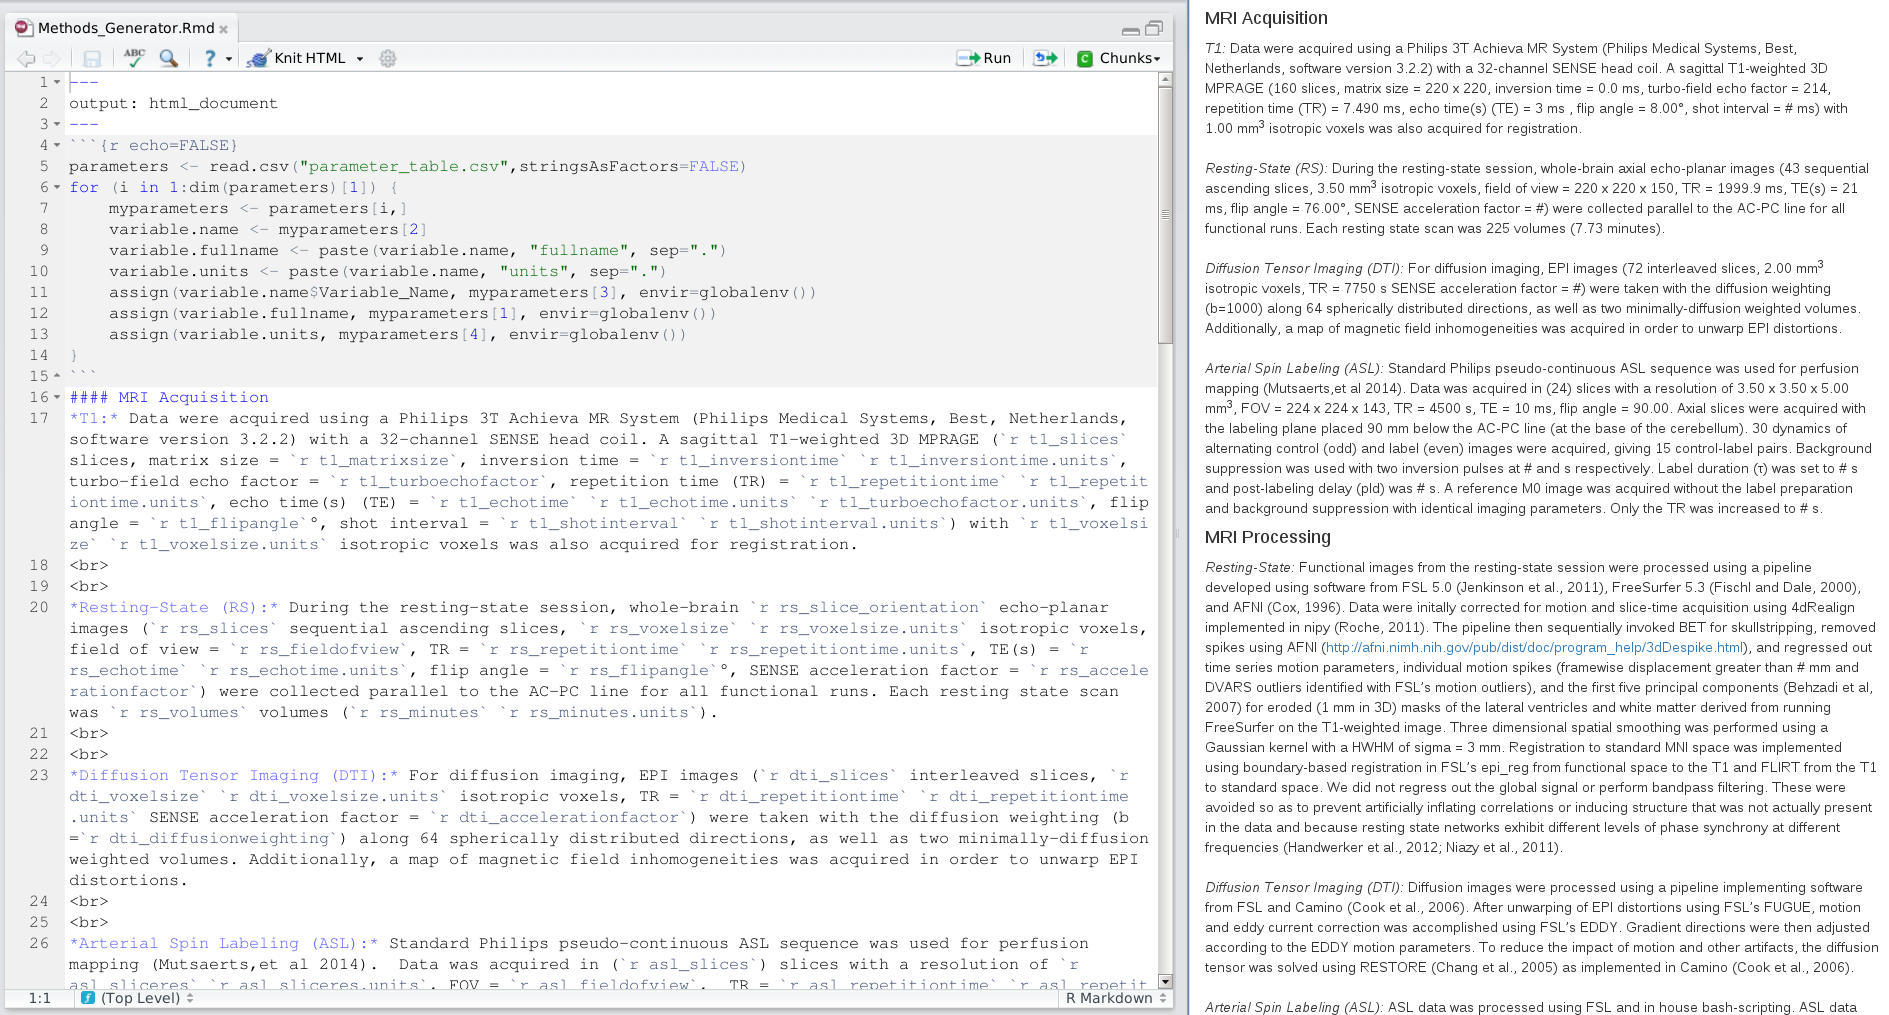
\includegraphics[width=7in]{../images/MethodsGenerator.png}
		\caption{Methods generation in R Markdown}
                \label{fig:methods}
	\end{center}
\end{figure}